\section{Распрацоўка аўтаматычнага разгортвання інфраструктуры для веб-сервісаў}

\subsection{Кароткае апісанне інфраструктуры}
\vspace{-1.5\baselineskip}
\begin{figure}[h!]
    \centering
    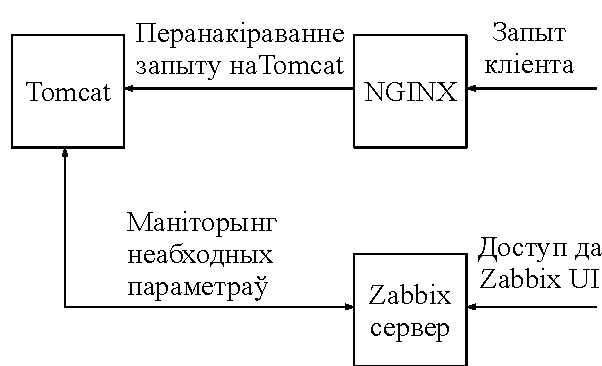
\includegraphics{diagram.pdf}
    \caption{Дыяграма інфраструктуры для веб-сервісаў}
    \label{figure:diagram} 
\end{figure}

\subsection{Інфраструктура як код}
Мадэль «Інфраструктура як код (IaC)», якую часам называюць «праграмуемай інфраструктурай», --- гэта мадэль, па якой працэс настройкі інфраструктуры аналагічны працэсу праграмавання праграмнага забеспячэння.

Інфраструктура як код дазваляе кіраваць віртуальнымі машынамі на праграмным узроўні. Гэта выключае неабходнасць ручной настройкі і абнаўленняў для асобных кампанентаў абсталявання. Інфраструктура становіцца адаптаванай да маштабавання. Адзін аператар можа выконваць разгортванне і кіраванне як адной, так і 1000 машынамі, выкарыстоўваючы адзін і той жа набор кода. Сярод гарантаваных пераваг інфраструктуры як кода - хуткасць, эканамічнасць і памяншэнне рызыкі.

\subsubsection{Канфігурацыйны файл разгортвання інфраструктуры.}
Канфігурацыйны файл разгортвання інфраструктуры прадстаўлены ў лістынку
\ref{lst:Vagrantfile}:

\lstinputlisting[caption={Зыходны код для разгортвання інфраструктуры},%
                            label={lst:Vagrantfile},%
                            language=Ruby]{Vagrantfile.rb}

У дадзенай канфігурацыі прадстаўлена апісанне 2 віртуальных машын,
Zabbix-Server і Zabbix-Agent.

Zabbix-Server --- віртуальная машына, на якой запушчаны Zabbix для
маніторынгу іншых сервісаў у сетцы.

Zabbix-Agent --- віртуальная машына, на якой запушчаны які-небудзь сервіс,
у дадзеным выпадку Tomcat, для абслугоўвання кліентаў.

Настройкі для Zabbix-Server і Zabbix-Agent прадастаўляюцца пры дапамозе
bash-скрыптаў zabbix-server.sh і zabbix-agent.sh адпаведна.
Канфігурацыйныя файлы настройкі будуць разгледжаны ў наступных раздзелах.

\subsubsection{Канфігурацыйны файл настройкі Zabbix-сервера.}
Канфігурацыйны файл настройкі Zabbix-сервера прадстаўлены ў лістынгу
\ref{lst:Zabbix-Server}:

\lstinputlisting[caption={Зыходны код для настройкі Zabbix сервера},%
                            label={lst:Zabbix-Server},%
                            language=Bash]{zabbix-server.sh}

Дадзены bash-скрыпт падчас разгортвання віртуальнай машыны
ўстанаўлівае і канфігурыруе для іх узаемадзеяння
базу даных MariaDB, Zabbix сервер, Apache сервер.

\subsubsection{Канфігурацыйны файл настройкі веб-сервера.}
Канфігурацыйны файл настройкі веб-сервера прадстаўлены ў лістынгу
\ref{lst:Zabbix-Agent}:

\lstinputlisting[caption={Зыходны код для настройкі веб-сервера},%
                            label={lst:Zabbix-Agent},%
                            language=Bash]{zabbix-agent.sh}

Дадзены bash-скрыпт падчас разгортвання віртуальнай машыны
ўстанаўлівае і канфігурыруе NGINX у якасці reverse-proxy сервера,
Tomcat для прадастаўлення веб-праграм кліенту, які "схаваны" за NGINX серверам.

У той жа час адбываецца настройка Tomcat сервіса для магчымасці адсочваць
java-параметры з удалённага хаста.

Пасля ўстаноўкі ўсіх неабходных кампанентаў запускаецца праграма 
<<zabbix-apy.py>>, які падключае дадзеную віртуальную машыну да
Zabbix сервера ў прыватнай сетцы.

\subsubsection{Python-праграма для аўтаматычнай рэгістрацыі Zabbix-агента.}
Python-праграма для аўтаматычнай рэгістрацыі Zabbix-агента на Zabbix серверы ў
прыватнай сетцы прадстаўлена ў лістынгу
\ref{lst:Python}:

\lstinputlisting[caption={Зыходны код для аўтаматычнай рэгістрацыі Zabbix-агента},%
                            label={lst:Python},%
                            language=Python]{zabbix-api.py}

Для змянення параметраў Zabbix сервера выкарыстоўваецца Zabbix API.

У дадзенай праграме выкарыстоўваюцца наступныя функцыі:
\begin{enumerate}
    \item post() -- другасная функцыя, якая выконвае запыт да Zabbix сервера і вяртае вынік аперацыі;
    \item is\_existed\_hostgroup() -- правярае ці існуе перададзеная група на Zabbix серверы;
    \item create\_hostgroup() -- стварае перададзеную групу на Zabbix серверы;
    \item get\_group\_id() --  вяртае id групы па імені групы;
    \item get\_ip\_address\_from\_server\_network() -- знаходзіць лакальны ip адрас машыны ў сетцы з Zabbix серверам;
    \item get\_template\_id() --  вяртае id шаблона па імені шаблона;
    \item is\_existed\_host() -- правярае ці існуе перададзеная імя хаста на Zabbix серверы;
    \item create\_host() -- рэгістрыруе машыну ў Zabbix серверы.
\end{enumerate}
